\section{Method}
\label{sec:method}

\subsection{Data} % (fold)
\label{sub:data}
\begin{itemize}
	\item \textbf{MNIST dataset} \cite{MNIST}, $\vec{X} = \curlies{\vec{X}\order{i}}^N_{i=1}$, of i.i.d. handwritten digits images with:
	\begin{itemize}
		\item \textbf{Training set} combining validation and training in 60000 images 
		\item \textbf{Test set} of 10000 images.
		\item Denotion of $\vec{X}\order{i} = \vec{x}$ for simplicity. 
	\end{itemize}
	\item \textbf{Reconstruction} $\tilde{\vec{X}}_{HR}$ of 
	\begin{itemize}
		\item $\vec{X}_{HR}: 28\times 28$ high-resolution (HR) images from
		\item $\vec{X}_{LR}: (28/d)\times (28/d)$ low-resolution (LR) images (downsampled by a factor of $d$)
	\end{itemize} 
\end{itemize}
% subsection data (end)

\subsection{Model} % (fold)
\label{sub:the_model}

%TODO: Tilføj diagram
% \begin{figure}
% 	\centering
	\usetikzlibrary{positioning}
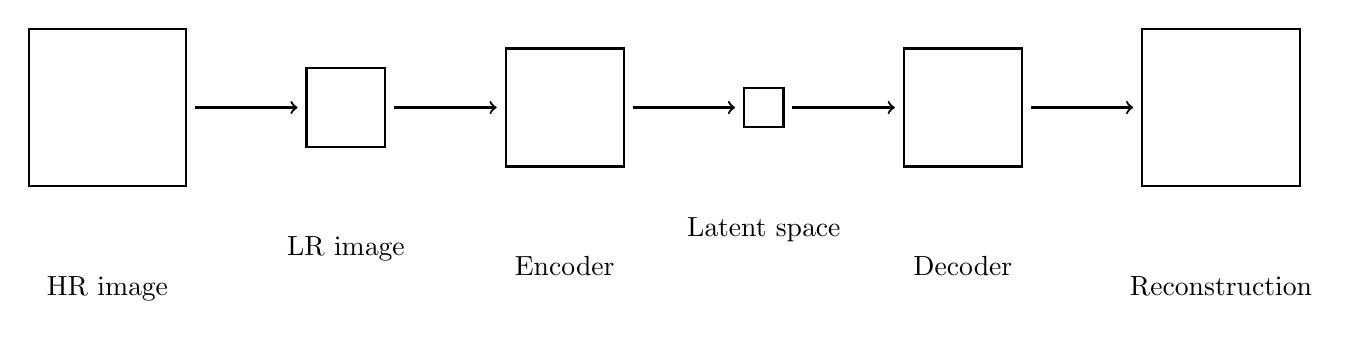
\begin{tikzpicture}[x = 1cm, y = 1cm, thick,
		image/.style={rectangle, draw, inner sep = 0pt, minimum size = 2 cm},
		network/.style={rectangle, draw, inner sep = 0pt, minimum size = 2 cm},
		arrow/.style={ ->, shorten <= 1 mm, shorten >= 1 mm}
	]
	
	\node[image, minimum size = 2 cm] (HR) at (0, 0) {};
	\node[below = of HR] {HR image};
	
	\node[image, minimum size = 1 cm, right = 1.5 cm of HR] (LR) {};
	\node[below = of LR] {LR image};
	
	\node[network, minimum size = 1.5 cm, right = 1.5 cm of LR] (encoder) {};
	\node[below = of encoder] {Encoder};
	
	\node[network, minimum size = 0.5 cm, right = 1.5 cm of encoder] (latent) {};
	\node[below = of latent] {Latent space};
	
	\node[network, minimum size = 1.5 cm, right = 1.5 cm of latent] (decoder) {};
	\node[below = of decoder] {Decoder};
	
	\node[image, minimum size = 2 cm, right = 1.5 cm of decoder] (reconstruction) {};
	\node[below = of reconstruction] {Reconstruction};
	
	\draw[arrow] (HR) -- (LR);
	\draw[arrow] (LR) -- (encoder);
	\draw[arrow] (encoder) -- (latent);
	\draw[arrow] (latent) -- (decoder);
	\draw[arrow] (decoder) -- (reconstruction);
	
\end{tikzpicture}

% 	\caption{Diagram of model.} 
% 	\label{fig:diagram}
% \end{figure}

\subsubsection{Downsampling} % (fold)
\label{ssub:downsampling}
\begin{itemize}
	\item \textbf{Mean pooling layer}
\end{itemize}
% subsubsection downsampling (end)

\subsubsection{Variational auto-encoder} % (fold)
\label{ssub:variational_auto_encoder}
\begin{itemize}
	\item \textbf{Goal}: Infer same structure from LR to HR. 
	\item \textbf{Solution}: Assume underlying probabilistic data generating process behind the production of digits. 
	\begin{itemize}
		\item \textbf{Decoding}: $\vec{x} \sim \dec{\vec{x}|\vec{z}}$ - Generate image from conditional distribution given
		\item \textbf{Encoding}: $\vec{z} \sim \enc{\vec{z}|\vec{x}}$ - Unobserved latent variable generated from the varitional approximation to the intractable true posterior $\dec{\vec{z}|\vec{x}}$
	\end{itemize}
	\item \textbf{Per-pixel loss-function}: `Free Energy' $\mathcal{L}\parens{\vec{\theta},\vec{\phi};\vec{x}}$:
	\begin{itemize}
		\item $\min_{\curlies{\vec{\theta},\vec{\phi}}} D_{KL}\parens{\enc{\vec{z}|\vec{x}}||\dec{\vec{z}|\vec{x}}}$: Minimize Kulback-Leibler divergence narrowed down by
		\item $\max_{\curlies{\vec{\theta},\vec{\phi}}}\mathcal{L}\parens{\vec{\theta},\vec{\phi};\vec{x}}$: maximize `Free Energy' as a variational lower bound.
		\item Derived from mean-field variational Bayes where the marginal log-likelihood can be decomposed like for the EM-algorithm and variational inference \cite[\S10.2]{Bishop2006}:
		\begin{equation}
			\log \dec{\vec{x}} = D_{KL}\left( \enc{\vec{z}|\vec{x}}||\dec{\vec{z}|\vec{x}}\right) + \mathcal{L}\left(\vec{\theta},\vec{\phi};\vec{x}\right)
		\end{equation} 
		\item \textbf{Variational lower bound}: non-negativity of the Kulback-Leibler divergence makes the Free energy $\mathcal{L}\parens{\vec{\theta},\vec{\phi};\vec{x}}$ a lower bound for the marginal log-likelihood:
			\begin{gather}
				\begin{split}
					\log \dec{\vec{x}} & \ge \mathcal{L}\left(\vec{\theta},\vec{\phi};\vec{x}\right) =
					\int \enc{\vec{z}|\vec{x}} \log \curlies*{ \frac{\dec{\vec{x},\vec{z}}}{\enc{\vec{z}|\vec{x}} } } \D{\vec{z}} \\
					& = -D_{KL}\parens{ \enc{\vec{z}|\vec{x}}||\dec{\vec{z}} } + \E_{\enc{\vec{z}|\vec{x}}} \brackets{\log \dec{\vec{x}|\vec{z}} }
				\end{split}
			\end{gather}
		\item First term: Regularizing $\vec{\phi}$ keeping the approximate posterior $\enc{\vec{z}|\vec{x}}$ close to the prior $\dec{\vec{z}}$. Has a differentiable analytical solution.
		\item Second term: Reconstruction error. Has a differentiable Monte Carlo estimate:
		\begin{equation}
			\E_{\enc{\vec{z}|\vec{x}}} \brackets{\log \dec{\vec{x}|\vec{z}} } \simeq \frac{1}{L}\sum^L_{l=1} \log \dec{\vec{x}|\vec{z}\order{l}}
		\end{equation}
		\item where a reparameterization trick is used for sampling $\vec{z}\order{l}= \vec{\mu} + \vec{\sigma} \odot \vec{\epsilon}\order{l}$ with white noise sample $\vec{\epsilon}\order{l} \sim \mathcal{N}(0,\vec{I})$
	\end{itemize}
	\item \textbf{Minibatch estimate}: $\frac{N}{M}\sum^{M}_{i=1}\tilde{\mathcal{L}}\parens{\vec{\theta},\vec{\phi};\vec{X}\order{i}}$
\end{itemize}
% subsubsection variational_auto_encoder (end)

\subsubsection{Neural Networks} % (fold)
\label{subsub:neural_networks}
\begin{itemize}
	\item Fully connected NN
	\item Convolutional NN 
\end{itemize}
% subsubsection neural_networks (end)


% subsection the_model (end)


% * Collection of data:
% 	* MNIST data
% * Methods (described to a level that others can reproduce the results):
% 	* Diagram (denote stochastic layers)
% 	* Downsampling (average pool layer)
% 	* VAE
% 		* Auto-encoder
% 		* Variational bound
% 	* Fully-connected neural network (NN)
% 	* Convolutional neural network (CNN) (*maybe*)
% * Experiments:
% 	* Reconstruction varying
% 		* downsampling factor
% 		* number of latent size
% 	* Super-resolution of home-made numbers


% Differentiation of L
% Output parameters (mu and sigma)